\appendix

\section{GPR Line of the test survey without interpretation}

\begin{figure}[H]
    \centering
    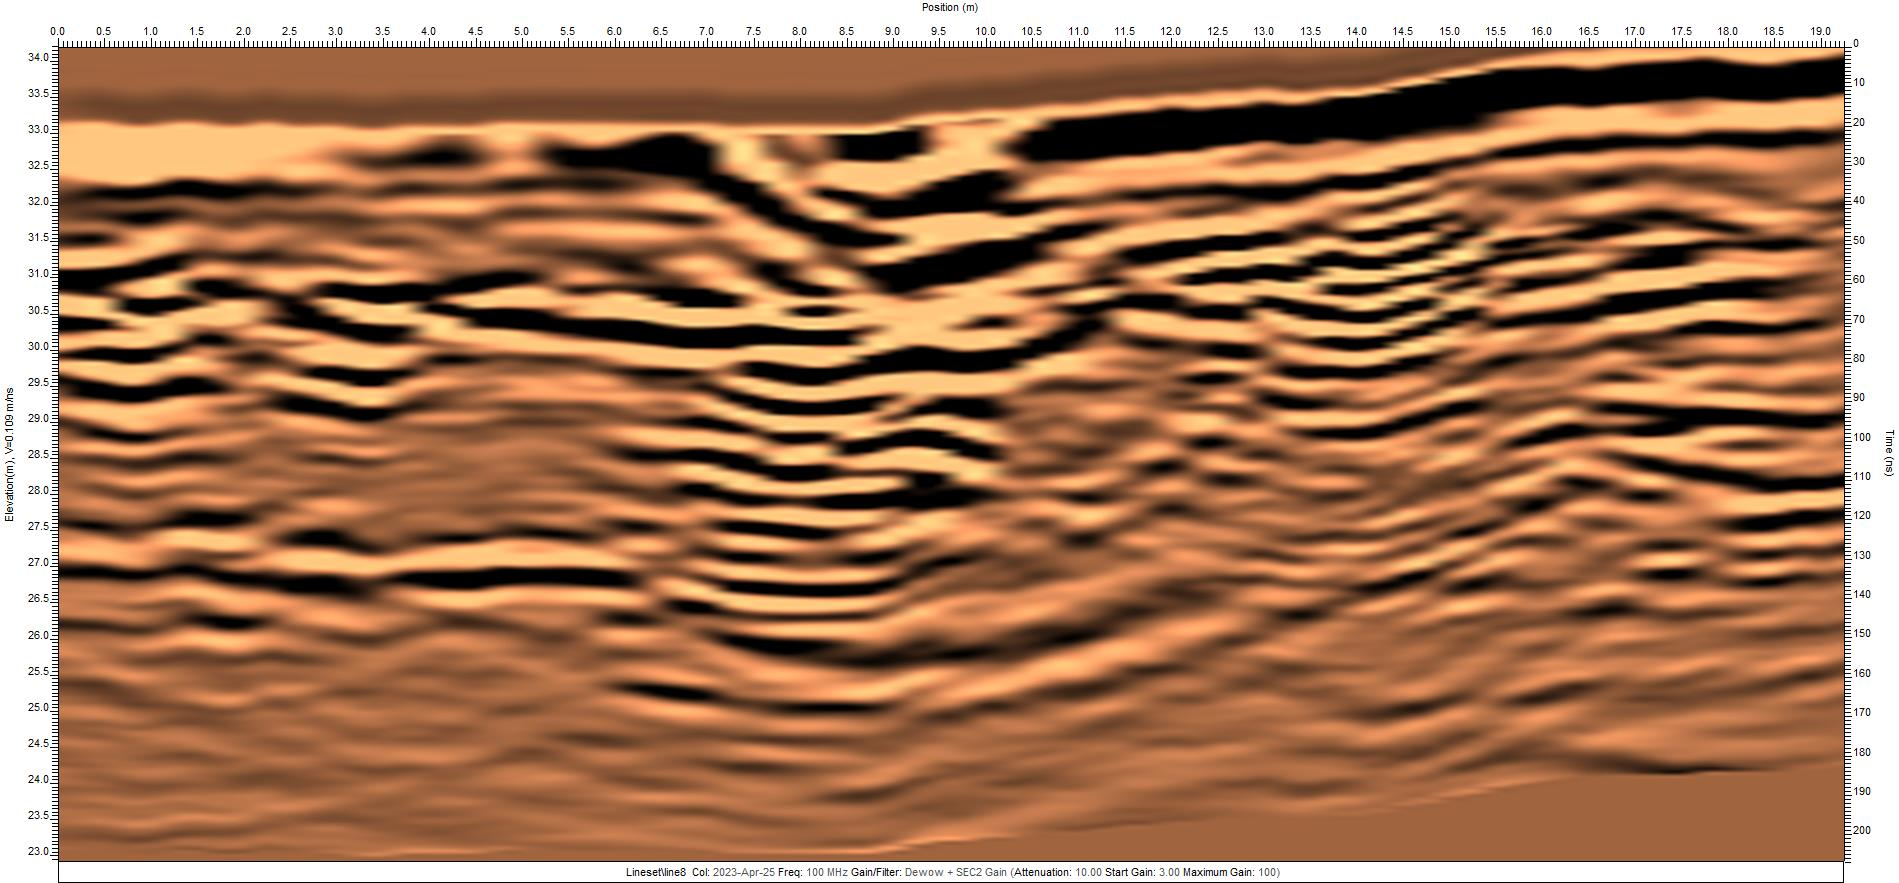
\includegraphics[width=\linewidth]{Images/00_Results/Test_line.jpg}
    \caption{Test Line}
    \label{fig:testLine_}
\end{figure}


\section{GPR Lines parallel to the slope without interpretation}

\begin{figure}[H]
    \centering
    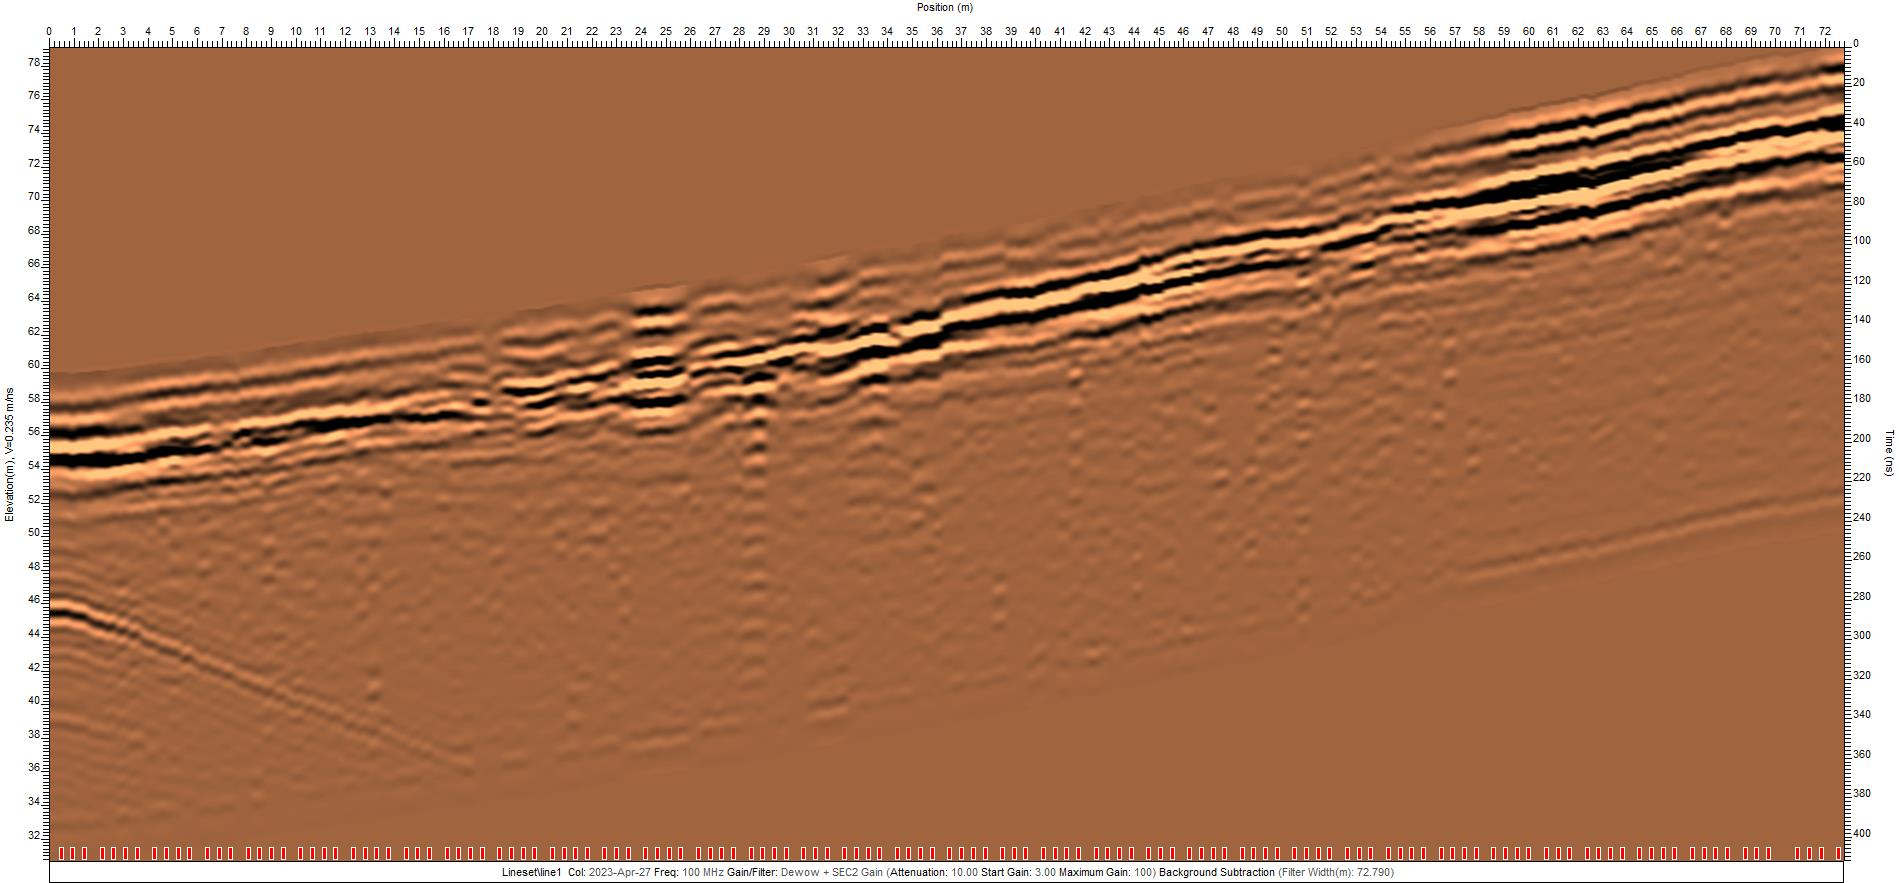
\includegraphics[width=\linewidth]{Images/00_Results/line1.jpg}
    \caption{Line 1}
    \label{fig:line1_}
\end{figure}

\begin{figure}[H]
    \centering
    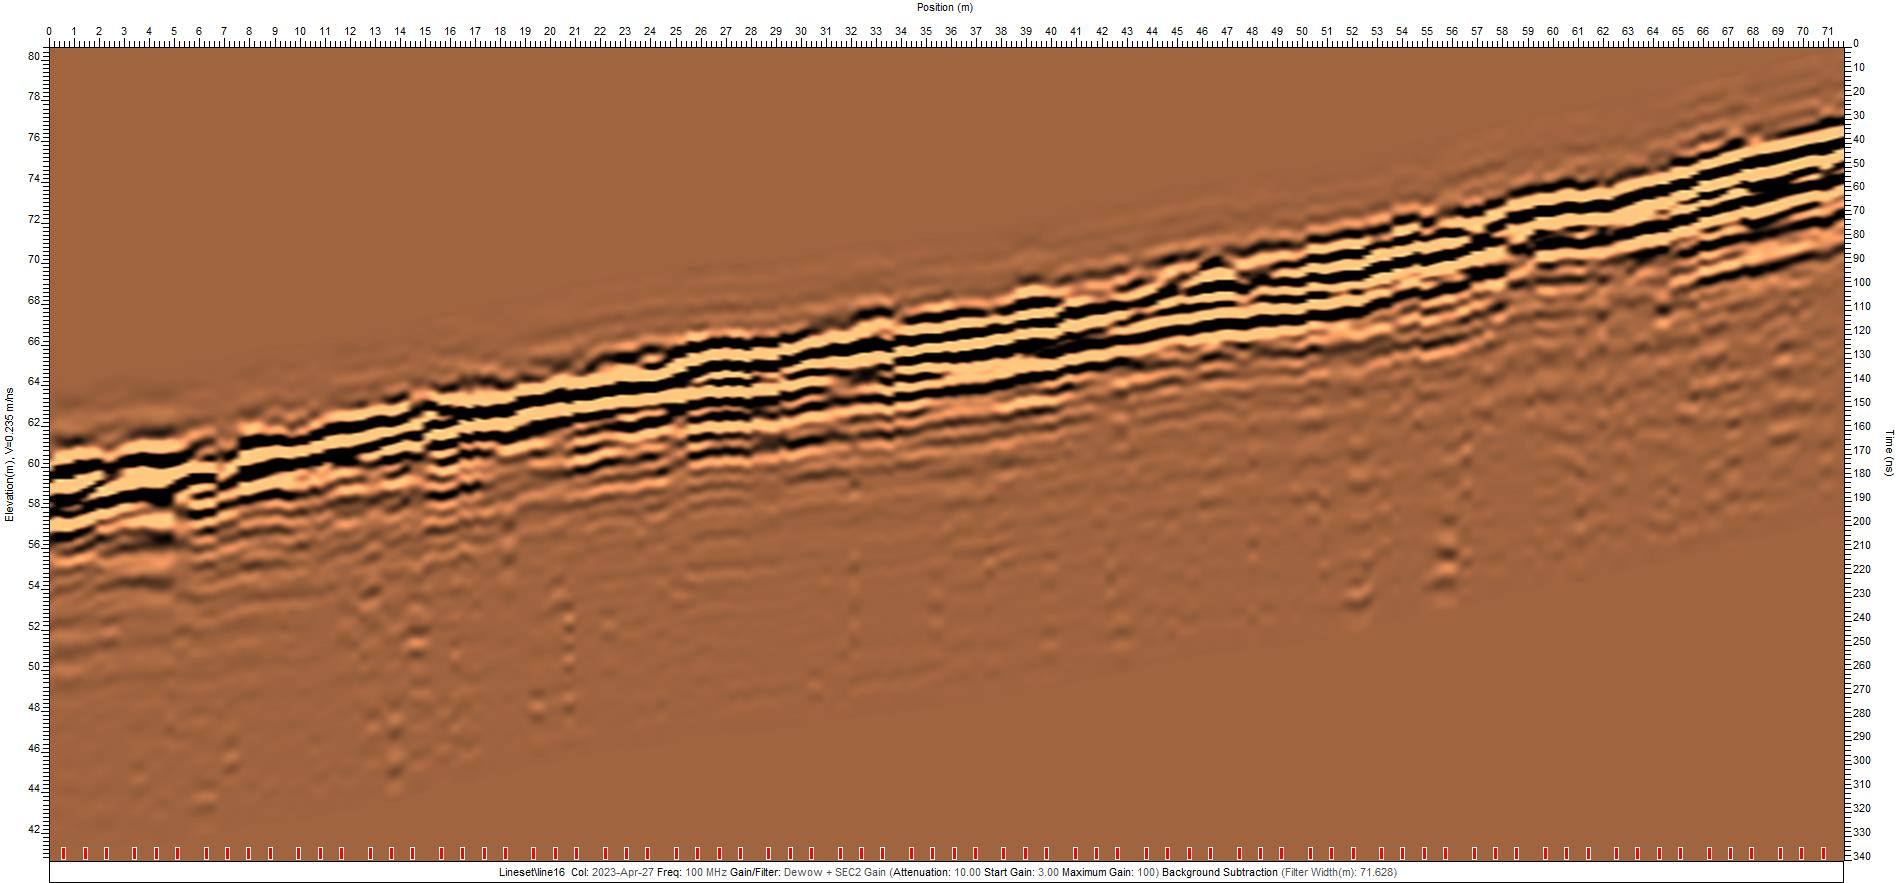
\includegraphics[width=\linewidth]{Images/00_Results/line16.jpg}
    \caption{Line 16}
    \label{fig:line16_}
\end{figure}

\begin{figure}[H]
    \centering
    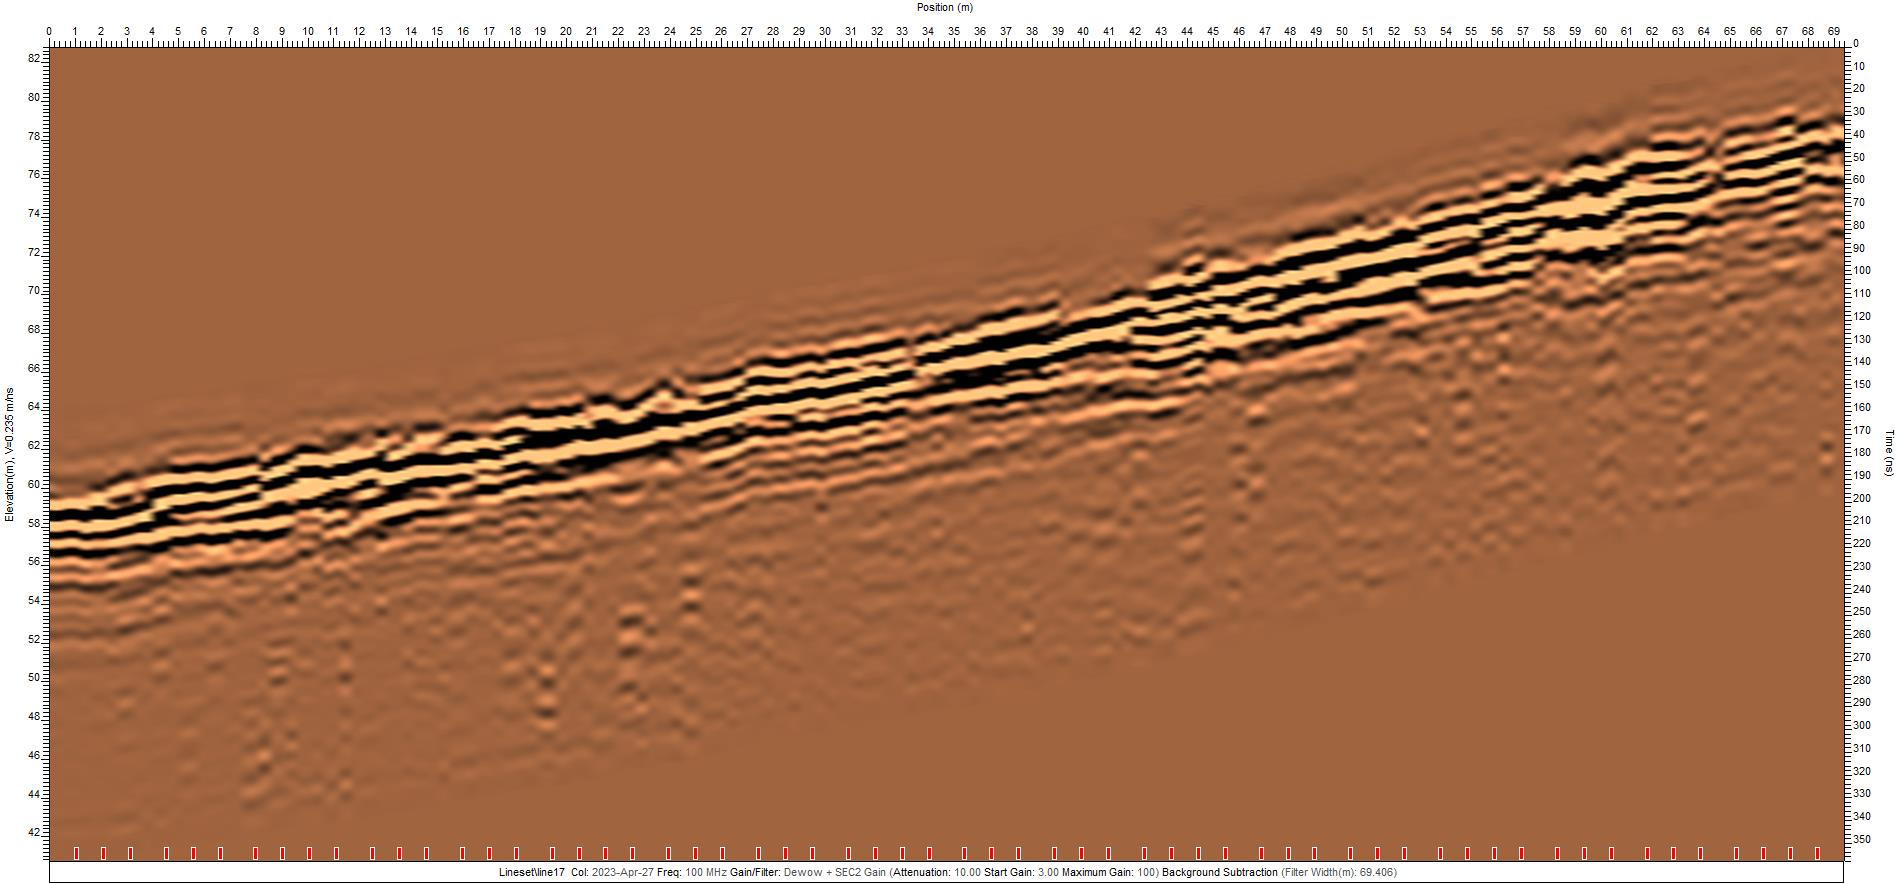
\includegraphics[width=\linewidth]{Images/00_Results/line17.jpg}
    \caption{Line 17}
    \label{fig:line17_}
\end{figure}

\begin{figure}[H]
    \centering
    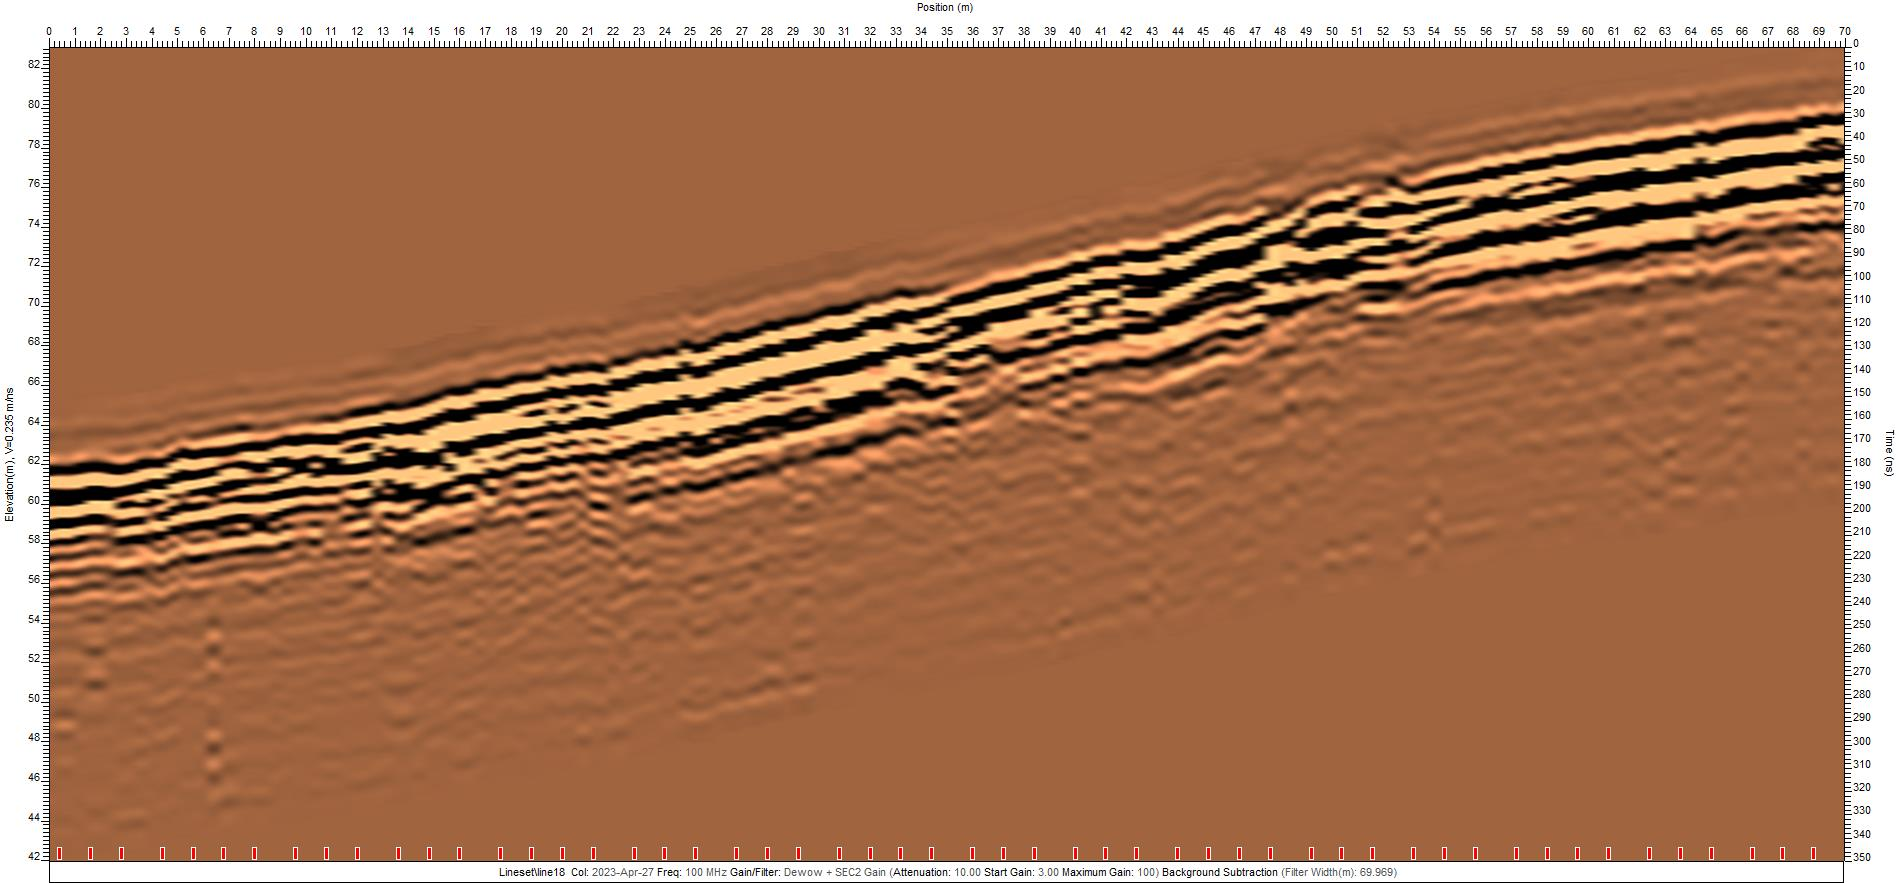
\includegraphics[width=\linewidth]{Images/00_Results/line18.jpg}
    \caption{Line 18}
    \label{fig:line18_}
\end{figure}

\begin{figure}[H]
    \centering
    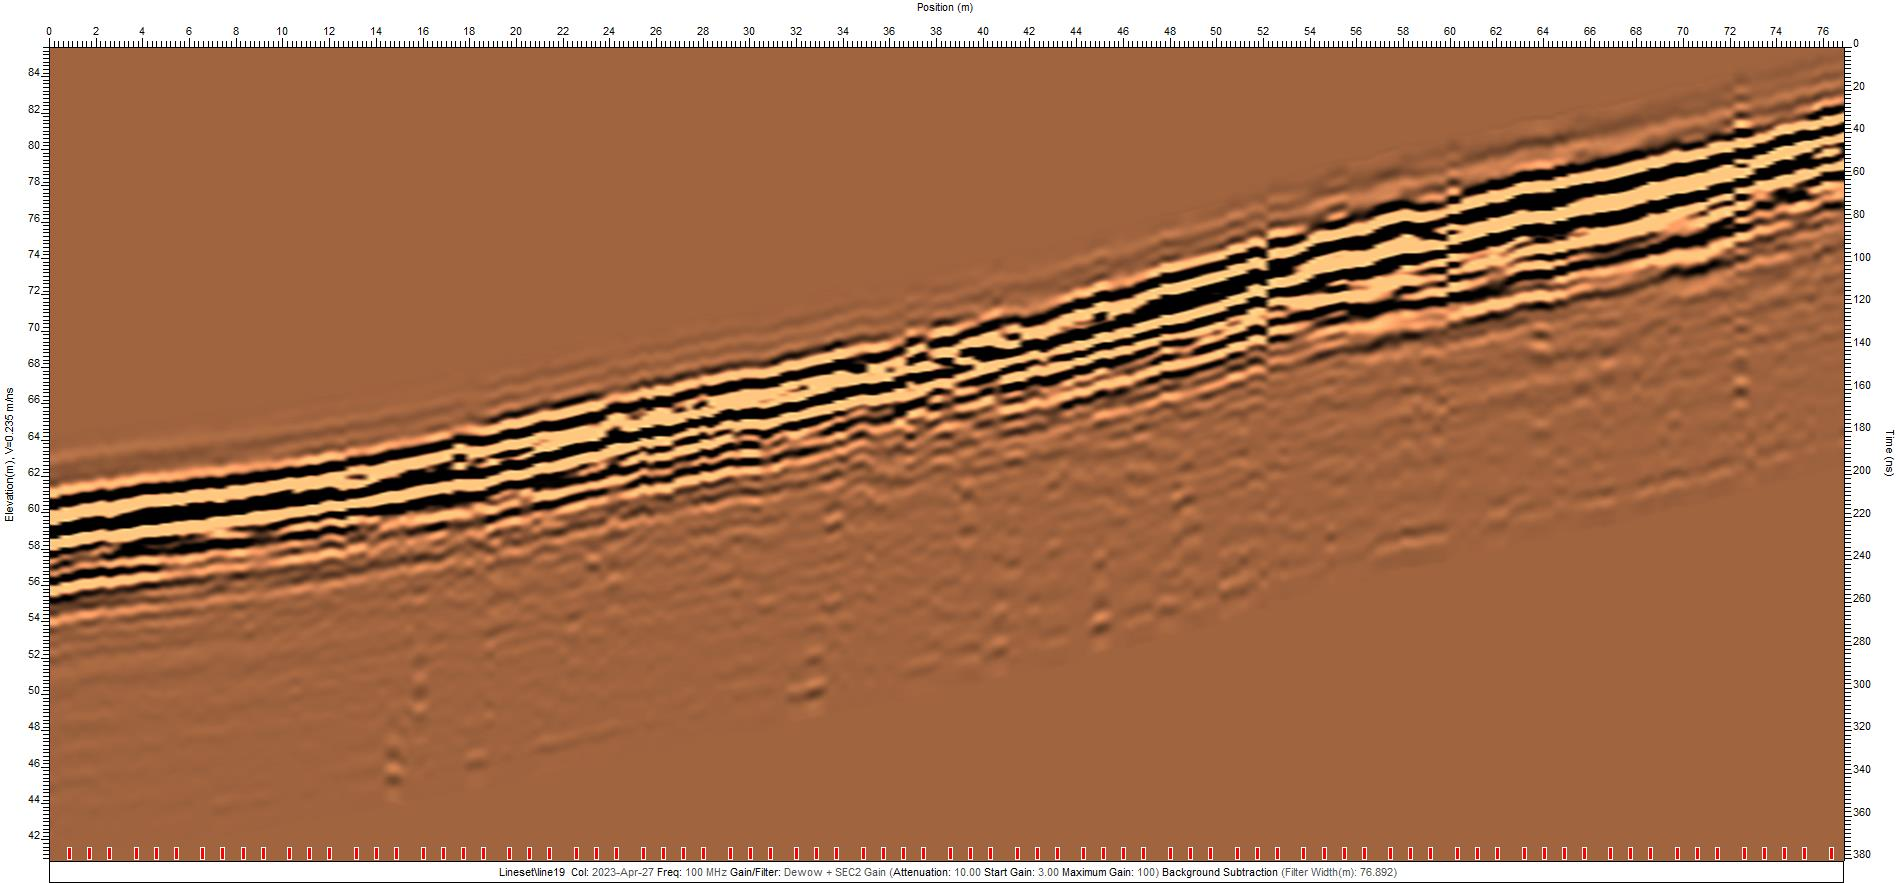
\includegraphics[width=\linewidth]{Images/00_Results/line19.jpg}
    \caption{Line 19}
    \label{fig:line19_}
\end{figure}

\begin{figure}[H]
    \centering
    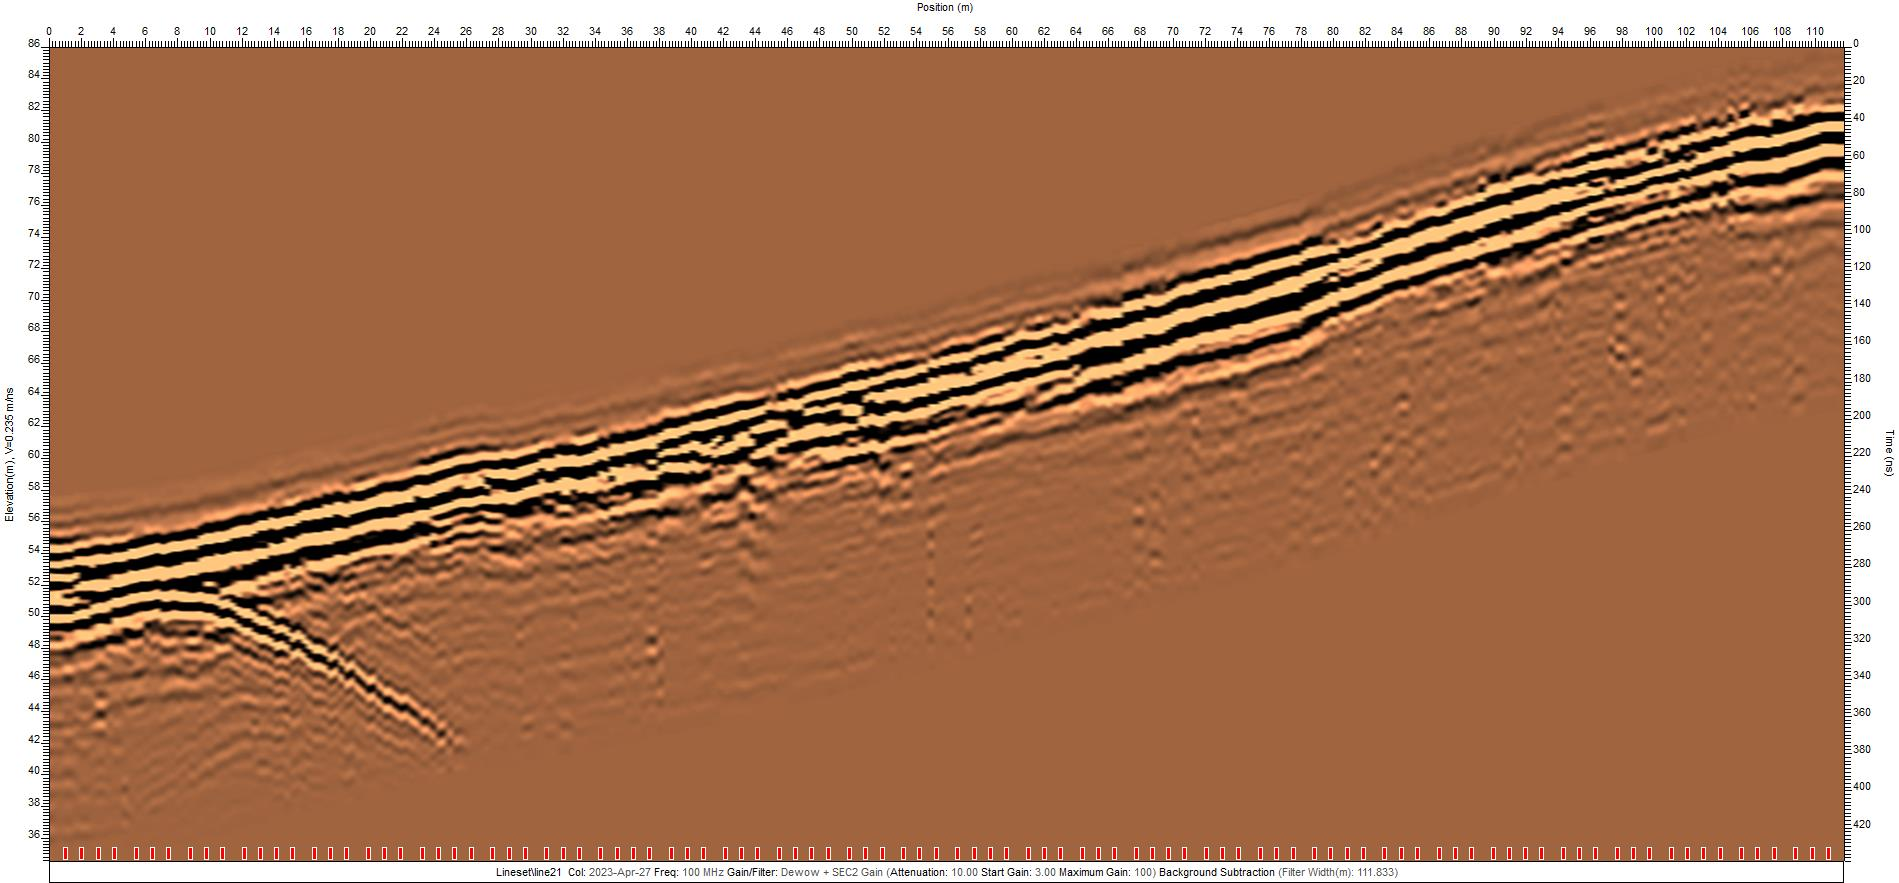
\includegraphics[width=\linewidth]{Images/00_Results/line21.jpg}
    \caption{Line 21}
    \label{fig:line21_}
\end{figure}

\section{GPR Lines perpendicular to the slope without interpretation}